\chapter{Prototype Implementation}
\label{Chapter4}
\lhead{Chapter 4. \emph{Prototype Implementation}}

In this chapter, we implement a prototype based on PTAM. It integrates the five methods in section \ref{VisualizationMethods}. A use case of this system is in section \ref{AUseCase}.

mobile device is equipped with a camera, GPS and gyrocompass devices. The camera lets the user take video from his own point of view. GPS and gyrocompass devices give the system the position and orientation of the mobile camera, respectively.


\section{System Architecture}

\subsection{Hardware}

\begin{itemize}
	\item The mobile device used is a SONY VAIO VGN-UX90PS, its specifications is in appendix \ref{AppendixA}. It has two built-in cameras. We use only the camera at the back as shown in figure \ref{fig:VAIOBack}, at 15fps@640x480.
	\item The gyrocompass attached is an InterSense InertiaCube3. It is one of the world's smallest inertial orientation reference system, its specifications is in appendix \ref{AppendixB}. The update rate is 180Hz, which eliminates tracker induced lag. It is connected to the mobile device with and RS322-USB adapter.
	\item The RTK-GPS system is shown in Figure [cite]. It is also connected to the mobile device with and RS232-USB adapter.
\end{itemize}

\subsection{Software}

The system does not use a server or any real surveillance camera. In place of those, 3D model of the building of the College of International Studies and the gymnasium (Figure [cite]), together with the hard coded geometry information about the virtual surveillance cameras are used.

The best visualization method is expected to be found visually and practically. A good visualization method can be the combination of many others at any extent. Thus, trial and error methodology can be applied here. To shorten the trial and error cycles, a good developmental environment of the preliminary system in this research, C language and OpenGL API \citep{Reference10} were used at first. Because both the language and the API are in too low level, the development speed was slow. Later, C language was replaced by Ruby language. The development speed was better but still slow. As as a result, it was concluded that the speed of the development is largely affected by the API rather than the language. Consequently, a higher level API has been adopted: OGRE \citep{Reference11}. OGRE, Object-Oriented Graphics Rendering Engine, is a scene-oriented, flexible 3D rendering engine written in C++ designed to make it easier and more intuitive for developers to produce applications utilizing hardware-accelerated 3D graphics. The class library abstracts all the details of using the underlying system libraries like Direct3D and OpenGL and provides an interface based on world objects and other intuitive classes.

\section{Viewing Modes}

The gyrocompass attached is an InterSense InertiaCube3. It is one of the world's smallest inertial orientation reference system, its specifications is in appendix \ref{AppendixB}. The update rate is 180Hz, which eliminates tracker induced lag. It is connected to the mobile device with and RS322-USB adapter.
	
\section{Prototype Characteristics}

Largely because the part to retrieve video images from the mobile camera is blocking, i.e. other parts of the program must wait while the images are being retrieved, the program is designed to be multithreaded. Its structure is shown in Figure [cite]. Visualization methods are programmed as visualizer plugins, so that the currently selected visualization method is changed by simply changing its corresponding plugin to another one. The thread to retrieve the image from the mobile camera runs at about 12fps@320x240, while the thread to display the final output image runs at about 10fps@640x480. This allows farther complex computation to be applied without noticeable delay and decrease in frame rates.

\section{History of this prototype}

The prototype described in the above sections is not the only decision choice we have made throughout this research. Previously, we have made others as described below.

\subsection{Hardware--Prototype with SONY VAIO VGN-UX90PS, Garmin GPSmap 60CSx, and InterSense InertiaCube3}

We have implemented a prototype with the architecture in figure \ref{fig:VAIOGPSGyro}. The GPS device specifications is in appendix \ref{AppendixD}. The GSP and gyrocompass devices provide position and orientation information of the mobile device. Together with the prebuilt CG information, we can overlay CG objects to visualize viewing fields of surveillance cameras. The update rate of the gyrocompass is 180Hz, which is high thus the orientation information is quite good. However, the GPS device error is about 10m, which affects badly the accuracy of the visualization. To improve the GPS device error, model-based tracking method as described in \citep{Reference13} method may be used.

\begin{figure}[htbp]
	\centering
	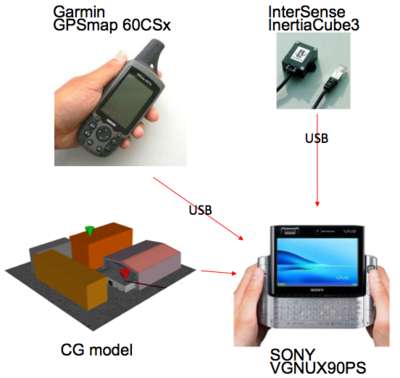
\includegraphics{./Primitives/vaio_gps_gyro.png}
	\rule{35em}{0.5pt}
	\caption[Prototype with SONY VAIO VGN-UX90PS, Garmin GPSmap 60CSx, and InterSense InertiaCube3]{Prototype with SONY VAIO VGN-UX90PS, Garmin GPSmap 60CSx, and InterSense InertiaCube3}
	\label{fig:VAIOGPSGyro}
\end{figure}

In the above prototype, we do not use GPS and gyrocompass devices. But GPS and gyrocompass devices can be used together with PTAM in the multi-sensor fusion \citep{Reference14} style, which may greatly improves the robustness of the system:

\begin{itemize}
	\item Initialization problem: the GPS and gyrocompass devices may provide initial position and orientation of the mobile device. Although the error of the GPS device is not small, in a large map it may help PTAM to reduce the search space.
	\item Quick movement: PTAM is image-based, thus it does not work well when the user quickly moves the mobile device. At this time, the gyrocompass may provide PTAM the orientation information because its update rate is high. Although the gyrocompass suffers from drifting error and needs to be continuously adjusted by the other sensors in the fusion, quick mobile device movement usually lasts only in a short time, thus gyrocompass may provide precious temporary information during this time.
\end{itemize}

\subsection{Software--Development environment}

Visualization methods are expected to be found experimentally and visually. Thus, trial and error methodology is applied here. To shorten the trial and error cycle, we need a good development environment which allows quick compiling, running and modifying.

At first we used C language and OpenGL API \citep{Reference10}. Because both the language and the API are in too low level, the development speed was slow. Later, C language was fully replaced by Ruby language. The development speed was better but still slow. It was concluded that the speed of the development is largely affected by the API rather than the language. Consequently, a higher level 3D rendering engine has been adopted: Irrlicht. Later, we read many reviews on the Internet that say that OGRE \citep{Reference11} is easier to use than Irrlicht, thus we migrated to OGRE. OGRE, Object-Oriented Graphics Rendering Engine, is a scene-oriented, flexible 3D rendering engine written in C++ designed to make it easier and more intuitive for developers to produce applications utilizing hardware-accelerated 3D graphics. The class library abstracts all the details of using the underlying system libraries like Direct3D and OpenGL and provides an interface based on world objects and other intuitive classes.

However, OGRE is generally used for creating 3D games thus contain too many features that we do not need. The framework forced us to write too much bloated code for the purpose of this research. As a result, we finally migrated to a combination of Ruby and C language with pure OpenGL API. At this time Ruby has grown to version 1.9. In this version the interpreter is replaced by a virtual machine, which boosts our Ruby program's speed to about 10x. It is ridiculously easy to write C extension for Ruby \citep{Reference15}. For program parts that need speed like networking and image processing, we write them as C extension for Ruby. For program parts that need trial-error or does not need speed like the user interface part, we write them in pure Ruby.
